\documentclass{sigkddExp}
\usepackage{longtable}
\usepackage{hyperref}


\usepackage{multicol}
\usepackage{titlesec}
\titlespacing*{\section}{0pt}{0.75em}{0.2em} % Adjusts space before and after section
\titlespacing*{\subsection}{0pt}{0.75em}{0.2em}
\titlespacing*{\subsubsection}{0pt}{0.75em}{0.2em}

\begin{document}

\title{Website Detection sing Machine Learning Techniques}

\numberofauthors{1}

\author{
%
% The command \alignauthor (no curly braces needed) should
% precede each author name, affiliation/snail-mail address and
% e-mail address. Additionally, tag each line of
% affiliation/address with \affaddr, and tag the
%% e-mail address with \email.
\alignauthor Nathan Opperman \\
       \affaddr{University of Pretoria}\\
       \affaddr{u21553832}\\
       \email{u21553832@tuks.co.za}
}

\date{30 October 2024}
\maketitle

\begin{abstract}
Text here...
\end{abstract}

\section{Introduction}
Phishing attacks have become a common issue, with cybercriminals leveraging deceptive tactics to steal sensitive information from users. One of the characteristics of such attacks is "Phishing Websites" that deceive victims by mimicking trusted entities such as banks or online shopping sites. One new method for detecting such websites is through the application of machine learning. Therefore, this research aims to investigate the challenge of phishing detection, focusing on the use of ML models that can help distinguish phishing sites from legitimate ones efficiently.
\subsection{Problem Statement}
\label{prob_statement}
Phishing is the malicious practice where attackers impersonate organizations, such as banks or retailers, through emails or messages, in an attempt to trick individuals into revealing sensitive information. Phishing websites, which mimic legitimate sites, play a crucial role in these attacks by luring users to enter their private information. It is quite clear that phishing attacks pose a significant threat and so there is a need for effective and time efficient detection methods to identify and quickly alert users to these threats.
\subsection{Research Questions}
This problem is expanded into the following research questions.
\subsubsection{What are the key features that can efficiently differentiate phishing websites from legitimate websites?}
\label{rq_1}
\subsubsection{What ML method will be best suited with efficiency and usability in mind?}
\label{rq_2}
\subsubsection{Is machine learning an affective approach for live detection?}
\label{rq_3}
\subsection{Research Objectives}
\label{research_objs}
With this project, I intend to develop and compare ML models, capable of accurately (and efficiently - speed) detecting these phishing websites to enhance cybersecurity. To evaluate these models I intend to develop a novel prototype detection mechanism that can detect phishing websites in near real-time.
\subsection{Methodology}
The methodology for this study involves several phases, starting with a literature survey to understand the current state of ML in phishing detection. Data collection and EDA follow, where relevant datasets are gathered, cleaned, preprocessed, and analyzed to ensure quality, and consistency and gain a general understanding of the data. Based on the findings from EDA, feature selection is performed to identify the most important variables that contribute to classification. To then optimize the chosen models, hyperparameter optimization is carried out. The main goal is to build an efficient classification model that accurately identifies phishing websites. Additionally, a basic prototype live detection mechanism is developed to apply the model in real-time environments, specifically the browser. Experimentation is then conducted to test the model through the prototype on various test cases. Finally, the results of experimentation and testing are then analyzed to determine the successes and weak points of the prototype/model.

\section{Literature Survey}
This literature study aims to explore and briefly explain referenced papers and other existing research on Phishing, machine learning for security applications, and existing baselines for ML in phishing website detection.
\subsection{Phishing}
A Phishing attack is described as a deceiving practice where the main idea of the attack is to impersonate a trustworthy entity in order to obtain unauthorized access to sensitive information for malicious \cite{10.5555/1071752.1071800, Ramzan2010}.

\vspace{1em}

The book \cite{Ramzan2010} further characterize phishing attacks using these three characteristics:

\begin{itemize}
	\item \textbf{A brand must be spoofed/impersonated}
	\item \textbf{A website must be involved}
	\item \textbf{Sensitive Information must be solicited}
\end{itemize}

The 2nd characteristic, phishing websites, is the main focus of this project.
\subsubsection{Phishing Websites}
Text here...
\subsubsection{Phishing Indicators}
Text here...
\subsection{Usability of ML for Security}
Text...
\subsubsection{Reliability}
Text...
\subsubsection{Trade-offs between Accuracy and Efficiency}
Text...
\subsubsection{Offline vs Online}
Text...
\subsection{Existing applications of ML in Phishing Detection}
Text here...
\subsubsection{Baselines}
Text here...
\subsubsection{Potential Gap}
Text here...

\section{Data Collection and EDA}
For this project, data was obtained from two distinct datasets, each for a specific and distinct purpose:
\begin{itemize}
	\item \textbf{Training:} The first dataset was sourced from a single, well-curated source for the purpose of training and initial evaluation of the model in an offline setting.
	\item \textbf{Live Detection:} The second dataset, used for real-time detection in a live environment (for the prototype), aggregates data from multiple sources, including user interactions in the browser and external APIs.
\end{itemize}
Each dataset has unique characteristics and requirements due to its purpose and source diversity, however both essentially share the same features. Instead, the source(s) and collection of data are dependent on the purpose. First, we look at the data collected for training purposes, and then data collected for live detection.
\subsection{Training: Phishing Websites Dataset}
The Phishing Websites dataset was utilized for the training and initial evaluation of various models. It was sourced from the UC Irvine Machine Learning Repository and was donated in 2015. The dataset contains a total of 11055 instances with 30 categorical ternary attributes derived from phishing indicators discussed and presented in \cite{6470857} as part of an effort to develop a group of features that are sound and effective in predicting phishing websites. Each attribute presents either one of three values: 1 (Legitimate), 0 (Suspicious), and -1 (Phishing). A highly summarized description of each feature is given in table \ref{feature-table}, however, each feature is discussed in more detail in \cite{6470857}. As mentioned, these features are indicators, each of which is intended to predict weather the website is a phishing website. Therefore, we can look at how affective each feature is at prediction though metrics such as accuracy, precision and recall \ref{fig:apr}.

\begin{figure*}[htbp]
  \centering
  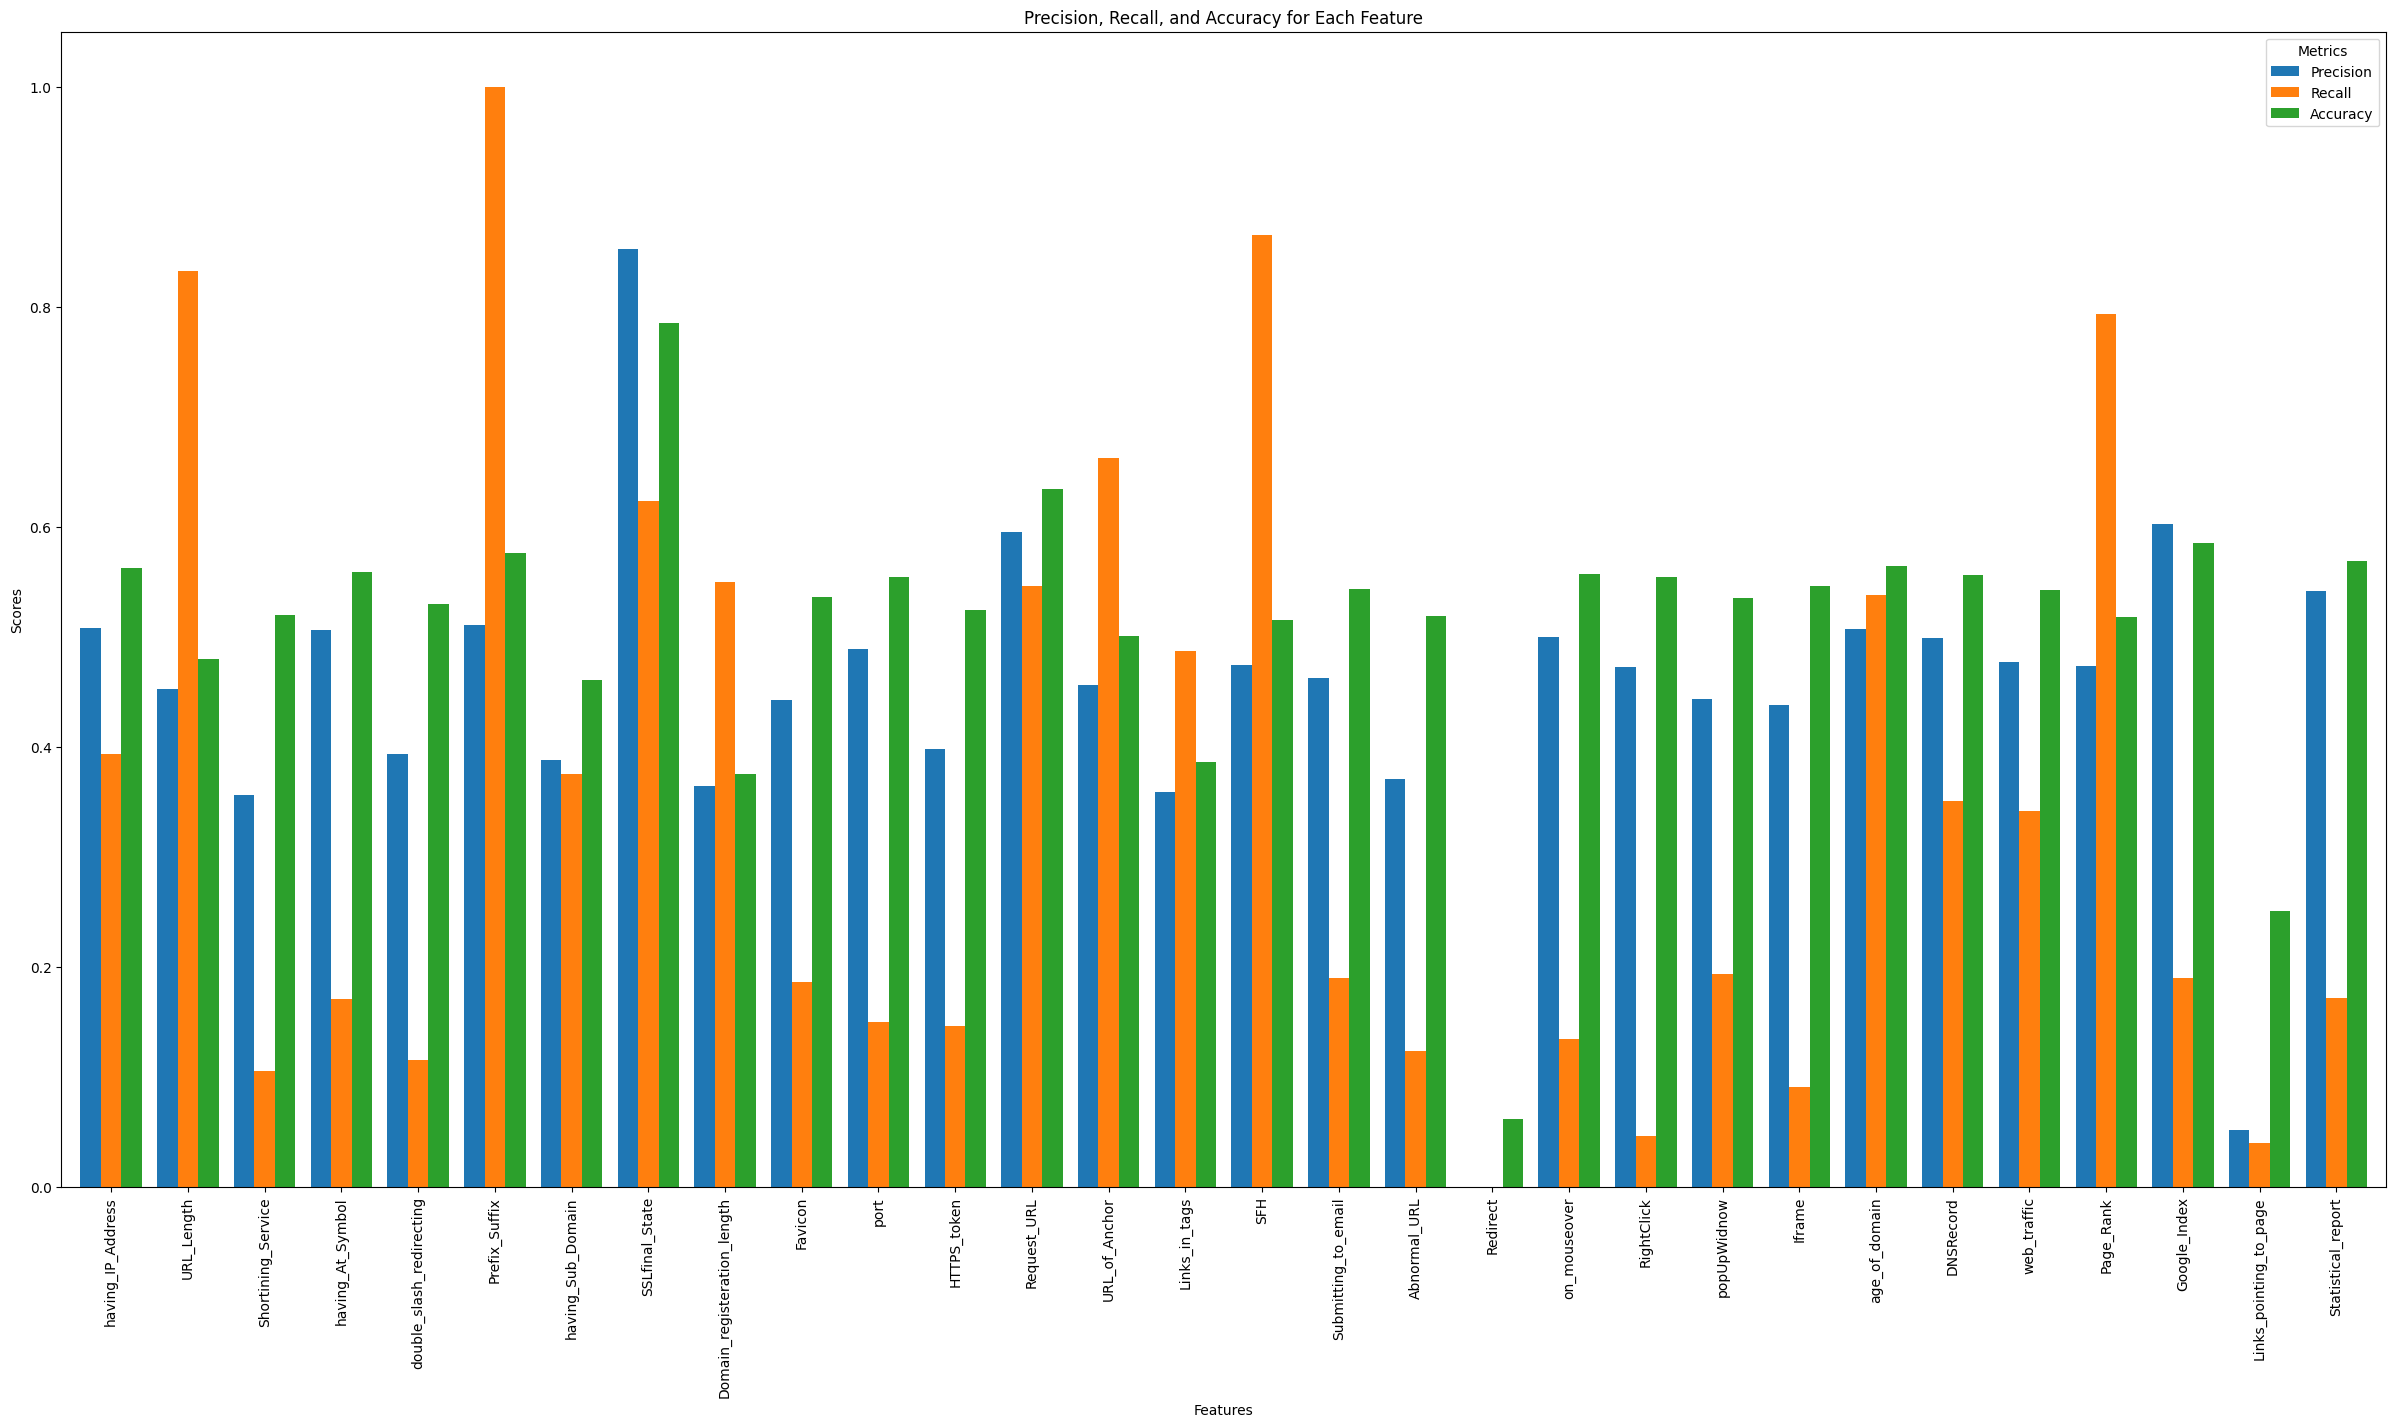
\includegraphics[width=0.6\textwidth]{./images/APR.png}
  \caption{Accuracy, Precision, and Recall of each indicator}
  \label{fig:apr}
\end{figure*}

\subsection{Live Detection: PhishTank}
The basis for the second form of data is PhishTank, specifically the urls of known active phishing websites published by PhishTank. A subset (10) of these websites will utilized during experimentation to gauge the performance of the live detection prototype (model). However, as mentioned the model is trained on the Phising Websites Dataset and so to apply the rules defined in \ref{feature-table} we utilize the DigitalRank, OpenPageRank, and Serp APIs along with the whois, ssl, requests, and BeutifulSoup Python libraries to determine the output for each indicator based on the url and html data collected. This is a dynamic approach to data collection that is a crucial aspect for live detection. While this data wont be used in training, it will play a role in feature selection. Another aspect to consider is cost, since these APIs have usage restrictions only a small subset of data will be utilized.

\subsection{Issues}
There are some issues regarding the Phishing Websites dataset that need to be discussed. Firstly the dataset is rather outdated (2015), this is especially concerning considering how cyber crime evolves. Firstly, Phishing websites are rather short-lived meaning that the websites used to extract these results are no longer online. Another issue is that some of the sources no longer exist, specifically the Alexa Internet Database, used to calculate website rankings, was terminated in 2022 and public PageRank scores, were discontinued in 2016. Fortunately, SimilarWeb (DigitalRank API) and OpenPageRank offer similar metrics that can be used. However, some of the more concerning issues have to do with the relevance of some of the indicators. A particularly outdated rule is the SSLFinal State rule requires that a certificate be older than one year, however, in March 2020 the CA/Browser forum voted that "after 1 September 2020 SHOULD NOT have a Validity Period greater than 397 days and MUST NOT have a Validity Period greater than 398 days" \cite{cabforum2020}. This is especially an issue when considering that 94.49\% of the websites collected from phishtank utilize HTTPS. Therefore, this rule will likely generate false positives during live detection. That said, the overall relevance and validity of the indicators is still present in modern day, however there effectiveness and reliability may have diminished.

\vspace{1em}

Another issue to consider, specifically for live detection is time efficiency. Since some of the indicators require external sources of data that must be acquired dynamically there is a time penalty, since we want to alert users quickly we must prioritize speed. Therefore indicators that take longer to determine are not encouraged.

\subsection{Feature Selection}
Based on the findings mentioned previously and the characteristics of the dataset I 
\begin{table}[h!]
\centering
\begin{tabular}{|p{2.5cm}|c|p{2.5cm}|c|}
\hline
\textbf{Top IG} & \textbf{IG} & \textbf{Top Comp} & \textbf{Comp} \\ \hline
sslfinal state             & 0.499  & url of anchor               & 0.690 \\ \hline
url of anchor              & 0.477  & sslfinal state              & 0.679 \\ \hline
prefix suffix              & 0.123  & prefix suffix               & 0.390 \\ \hline
web traffic                & 0.115  & having\_sub\_dom           & 0.378 \\ \hline
having\_sub\_dom          & 0.110  & links in tags               & 0.325 \\ \hline
links in tags              & 0.047 & request url                 & 0.324 \\ \hline
request url                & 0.047 & sfh                         & 0.317 \\ \hline
sfh                        & 0.037 & domain\_reg\_len  & 0.316 \\ \hline
domain\_reg\_len & 0.037 & age of domain               & 0.294 \\ \hline
google index              & 0.012  & having ip address           & 0.290 \\ \hline
\end{tabular}
\caption{Top 10 Features Ranked by Information Gain and Composite Score}
\label{table:feature_ranking}
\end{table}
 
\section{Hyperparameter Optimization}
Text here...

\section{Results}
Text here...

\section{Evaluation}
Text here...

\section{Conclusion}
Text here...

%
% The following two commands are all you need in the
% initial runs of your .tex file to
% produce the bibliography for the citations in your paper.
\bibliographystyle{abbrv}
\bibliography{sigproc}  % sigproc.bib is the name of the 
\newpage
\appendix
\section{Phishing Website Features}

\begin{table}[h!]
\centering
\begin{tabular}{|p{3cm}|l|p{8cm}|l|l|l|l|}
\hline
\textbf{Feature} & \textbf{Range} & \textbf{Rule} & \textbf{-1} & \textbf{0} & \textbf{1} & \textbf{Acc (\%)} \\
\hline
\textbf{having IP Address} & `-1, 1` & If the domain part has an IP address → \textbf{-1}, Otherwise → \textbf{1} & 3793 & 0 & 7262 & 56.228 \\
\hline
\textbf{URL Length} & `1, 0, -1` & If URL length < 54 → \textbf{1}, If URL length >= 54 and <= 75 → \textbf{0}, Otherwise → \textbf{-1} & 8960 & 135 & 1960 & 47.9692 \\
\hline
\textbf{Shortening Service} & `1, -1` & If using TinyURL or similar services → \textbf{-1}, Otherwise → \textbf{1} & 1444 & 0 & 9611 & 51.9313 \\
\hline
\textbf{having At Symbol} & `1, -1` & If URL contains "@" symbol → \textbf{-1}, Otherwise → \textbf{1} & 1655 & 0 & 9400 & 55.8661 \\
\hline
\textbf{double slash redirecting} & `-1, 1` & If "//" appears in the URL after position 7 → \textbf{-1}, Otherwise → \textbf{1} & 1429 & 0 & 9626 & 52.9353 \\
\hline
\textbf{Prefix Suffix} & `-1, 1` & If URL has hyphens/dots at start or end → \textbf{-1}, Otherwise → \textbf{1} & 9590 & 0 & 1465 & 57.5577 \\
\hline
\textbf{having Sub Domain} & `-1, 0, 1` & More than one subdomain → \textbf{-1}, Single subdomain → \textbf{0}, Otherwise → \textbf{1} & 3363 & 3622 & 4070 & 46.0968 \\
\hline
\textbf{SSLfinal State} & `-1, 1, 0` & Invalid or missing SSL certificate → \textbf{-1}, Valid but not fully secure SSL → \textbf{0}, Otherwise → \textbf{1} & 3557 & 1167 & 6331 & 78.5256 \\
\hline
\textbf{Domain registration length} & `-1, 1` & If domain registered for less than 6 months → \textbf{-1}, Otherwise → \textbf{1} & 7389 & 0 & 3666 & 37.5215 \\
\hline
\textbf{Favicon} & `1, -1` & If favicon exists and is legitimate → \textbf{1}, Otherwise → \textbf{-1} & 2053 & 0 & 9002 & 53.5685 \\
\hline
\textbf{port} & `1, -1` & If using standard ports → \textbf{1}, Otherwise → \textbf{-1} & 1502 & 0 & 9553 & 55.3867 \\
\hline
\textbf{HTTPS token} & `-1, 1` & Checks if "https" is present in the URL and used correctly. If "https" is absent or inconsistently used → \textbf{-1}, Otherwise → \textbf{1} & 1796 & 0 & 9259 & 52.3835 \\
\hline
\textbf{Request URL} & `1, -1` & Legitimate URL in request → \textbf{1}, Otherwise → \textbf{-1} & 4495 & 0 & 6560 & 63.4283 \\
\hline
\textbf{URL of Anchor} & `-1, 0, 1` & Misleading or missing anchor text → \textbf{-1}, Generic anchor text → \textbf{0}, Otherwise → \textbf{1} & 3282 & 5337 & 2436 & 50.0407 \\
\hline
\textbf{Links in tags} & `1, -1, 0` & No links or links to legitimate sites → \textbf{1}, Links to suspicious sites → \textbf{-1}, Otherwise → \textbf{0} & 3956 & 4449 & 2650 & 38.6251 \\
\hline
\textbf{SFH} & `-1, 1, 0` & SFH points to a non-legitimate site → \textbf{-1}, SFH is a generic form handler → \textbf{0}, Otherwise → \textbf{1} & 8440 & 761 & 1854 & 51.5152 \\
\hline
\textbf{Submitting to email} & `-1, 1` & Form submission via email → \textbf{-1}, Otherwise → \textbf{1} & 2014 & 0 & 9041 & 54.3193 \\
\hline
\textbf{Abnormal URL} & `-1, 1` & Unusual characters or patterns → \textbf{-1}, Otherwise → \textbf{1} & 1629 & 0 & 9426 & 51.8860 \\
\hline
\textbf{Redirect} & `0, 1` & Redirects to another domain → \textbf{-1}, No redirection → \textbf{1}, Otherwise → \textbf{0} & 0 & 9776 & 1279 & 6.12393 \\
\hline
\textbf{on mouseover} & `1, -1` & Suspicious behavior on mouseover → \textbf{-1}, Otherwise → \textbf{1} & 1315 & 0 & 9740 & 55.6852 \\
\hline
\textbf{RightClick} & `1, -1` & Right-click disabled → \textbf{-1}, Otherwise → \textbf{1} & 476 & 0 & 10579 & 55.4591 \\
\hline
\textbf{popUpWindow} & `1, -1` & Unsolicited pop-ups → \textbf{-1}, Otherwise → \textbf{1} & 2137 & 0 & 8918 & 53.4962 \\
\hline
\textbf{Iframe} & `1, -1` & Iframes with external content → \textbf{-1}, Otherwise → \textbf{1} & 1012 & 0 & 10043 & 54.5545 \\
\hline
\textbf{age of domain} & `-1, 1` & If the domain age is below a threshold (e.g., 6 months) → \textbf{-1}, Otherwise → \textbf{1} & 5189 & 0 & 5866 & 56.3727 \\
\hline
\textbf{DNSRecord} & `-1, 1` & Missing or suspicious DNS records → \textbf{-1}, Otherwise → \textbf{1} & 3443 & 0 & 7612 & 55.6309 \\
\hline
\textbf{web traffic} & `-1, 0, 1` & Low or no web traffic → \textbf{-1}, Moderate web traffic → \textbf{0}, Otherwise → \textbf{1} & 2655 & 2569 & 5831 & 54.2469 \\
\hline
\textbf{Page Rank} & `-1, 1` & Low or no page rank → \textbf{-1}, Otherwise → \textbf{1} & 8201 & 0 & 2854 & 51.7956 \\
\hline
\textbf{Google Index} & `1, -1` & Indexed by Google → \textbf{1}, Otherwise → \textbf{-1} & 1539 & 0 & 9516 & 58.5436 \\
\hline
\textbf{Links pointing to page} & `1, 0, -1` & Many legitimate links → \textbf{1}, Few links → \textbf{0}, No or bad links → \textbf{-1} & 548 & 6156 & 4351 & 25.0384 \\
\hline
\textbf{Statistical report} & `1, 0, -1` & Report generated and valid → \textbf{1}, Otherwise → \textbf{0 or -1} & 1550 & 0 & 9505 & 56.8521 \\
\hline
\textbf{Result} & `-1, 1` & Final classification is phishing → \textbf{-1}, Otherwise → \textbf{1} & 4898 & 0 & 6157 & N/A\\
\hline
\end{tabular}
\caption{Feature Summary Table for Phishing Websites}
\label{feature-table}
\end{table}
\end{document}
